\section{Relacje binarne}

\begin{center}
\begin{table}[h]
    \centering
    \begin{tabular}{|c|c|c|c|}
    \hline
    $R_2$ & a & b & c \\ \hline
    a & 1 & 1 & 0 \\ \hline
    b & 0 & 0 & 0 \\ \hline
    c & 0 & 0 & 0 \\ \hline
    \end{tabular}
\end{table}

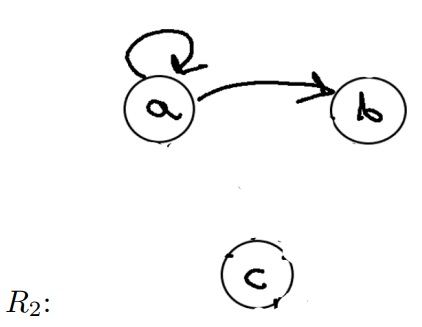
\includegraphics[scale=0.5]{img/grafR2.png}
\end{center}

\subsection{Własności relacji}

Niech dana będzie relacja binarna na $ R \subseteq X \times X $

Za przykładowe uniwersum posłuży nam zbiór $U = \{ a, b, c, d \} $ \\

Własności relacji i ich warunki

\begin{itemize}
    \item Zwrotna -- $\forall x \in X (<x,x> \in R)$
    
    Aby było zwrotna w relacji \textbf{musi} znaleźć się $ \{ <a, a>, <b, b>, <c, c>, <d, d> \} $

    \item Przeciwsymetryczna (asymetryczna, silnie antysymetryczna) -- $\forall x \in X(\neg <x, x> \in R) $
    
    Aby była przeciwzwrotna to w relacji \textbf{nie może} znaleźć się \textbf{żadna} z tych par \linebreak 
    $ <a, a>, <b,b>, <c,c>, <d,d> $

    \item Antysymetryczna (słabo antysymetryczna) -- $ \forall x \forall y \in X(((x, y) \in R \ \land \ (y, x) \in R) \Rightarrow x = y) $
    
    \item Symetryczna -- $ \forall x \forall y \in X(<x,y> \in R \Rightarrow <y,x> \in R) $
    
    Aby była symetryczna to \textbf{każda istniejąca para w relacji} musi mieć swoje lustrzane odbicie. Na przykład:
    $ \{ <a,b>, <b,a>, <a, a>, <b,c>, <c,b> \} $

    \item Asymetryczna -- $\forall x \forall y \in X((<x,y> \in R \land (y,x) \in R) \Rightarrow x=y) $
    
    \item Przeciwsymetryczna -- $\forall x \forall y \in X(<x,y> \in R) \Rightarrow \neg <y,x> \in R) $
    
    \item Spójna -- $\forall x \forall y \in X(< x, y >\in R \lor < y, x >\in R) $ -- strzałki muszą być w dwie strony
    
    \item Tolerancyjna, podobieństwa -- tylko wtedy gdy jest zwrotna i symetryczna
    
    \item Przechodnia -- $\forall x \forall y \forall z (<x,y> \in R \ \land <y,z> \in R \Rightarrow \ <x,z> \in R)$
    
    Na chłopski rozum -- relacja jest przechodnia w sytuacji gdy zawsze - "jeśli można przejść z $a$ do $b$ i z $b$ można przejść do $c$
    to też można przejść z $a$ do $c$. Trzeba uważać na to, że definicja jest implikacją. Relacja $ R = \{ <a,a> \} $ jest przechodnia.

    $ R = \{ <a,b>, <b,a> \} $ -- nie jest zwrotna bo brakuje $ \{ <a,a>, <b,b> \} $

    \item Równoważności -- musi być zwrotna, symetryczna i przechodnia
\end{itemize}

\subsection{Działania na relacjach}

\begin{enumerate}
    \item Dopełnienie : $ \overline{R} = X^2 \backslash R $
    
    Czyli wszystkie pary, których nie ma w oryginalnej relacji

    \item $ R \cup Q = \{ <x,y> \in R \ \lor <x,y> \in Q \} $
    \item $ R \cap Q = \{ <x,y> \in R \ \land <x,y> \in Q \} $
    \item $ R^{-1} = \{<y,x> \in R\} $ -- czyli odwracamy strzałki
    \item $ R^{=} = R \cup \{<x,x> : x \in X\} $ -- sprawiamy, że \textbf{wszędzie} muszą być pętelki
    \item $ R^{\neq} = R \backslash \{ <x,x> : x \in X \} $ -- przeciwieństwo z pkt. 5 -- \textbf{usuwamy wszędzie} pętelki
    \item $ R^+ $ -- dopełnienie tranzytywne -- sprawiamy, że relacja staje się przechodnia jeśli nią jeszcze nie jest
    
    Na przykład -- $ R = \{ <a,b>, <b,a> \} $ \ to \ $ R^+ = R \cup \{ <a,a>, <b,b> \} $ 

    \item $ R^- $ -- redukt tranzytywny
    
    Algorytm :
    \begin{enumerate}
        \item Znajdź cykle, jeśli jakiś element został już użyty w jakimś cyklu, \textbf{nie używaj go ponownie}
        \item Jeśli jakiś cykl powstał tylko dlatego, że była na nim pętelka, to dodaj na nim pętelkę
        \item Usuń z nowo powstałego grafu niepotrzebne strzałki, czyli takie, które duplikują istniejące już przejścia
        \item Wypisz już z powrotem graf tylko z oryginalnymi elementami, z usuniętymi niepotrzebnymi strzałlkami
    \end{enumerate}

    Ważne : jeśli jakiś element nie jest z żadnym elementem w cyklu to jest on "w cyklu z samym sobą"
    
    \begin{center}
        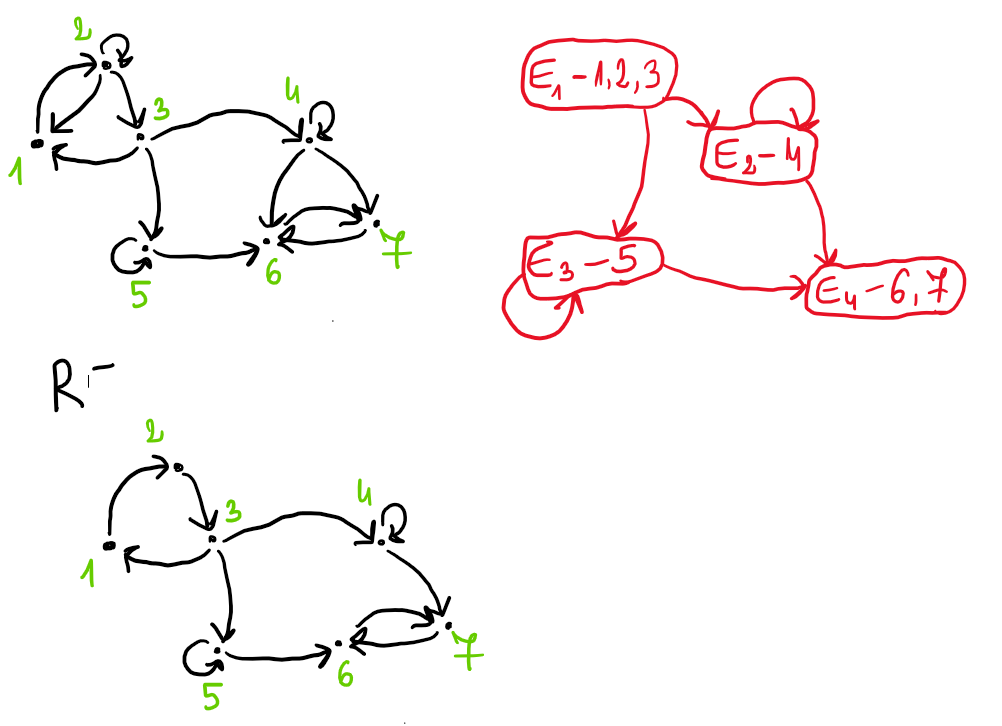
\includegraphics[scale=0.5]{img/redukt.png}

        Przykład 1

        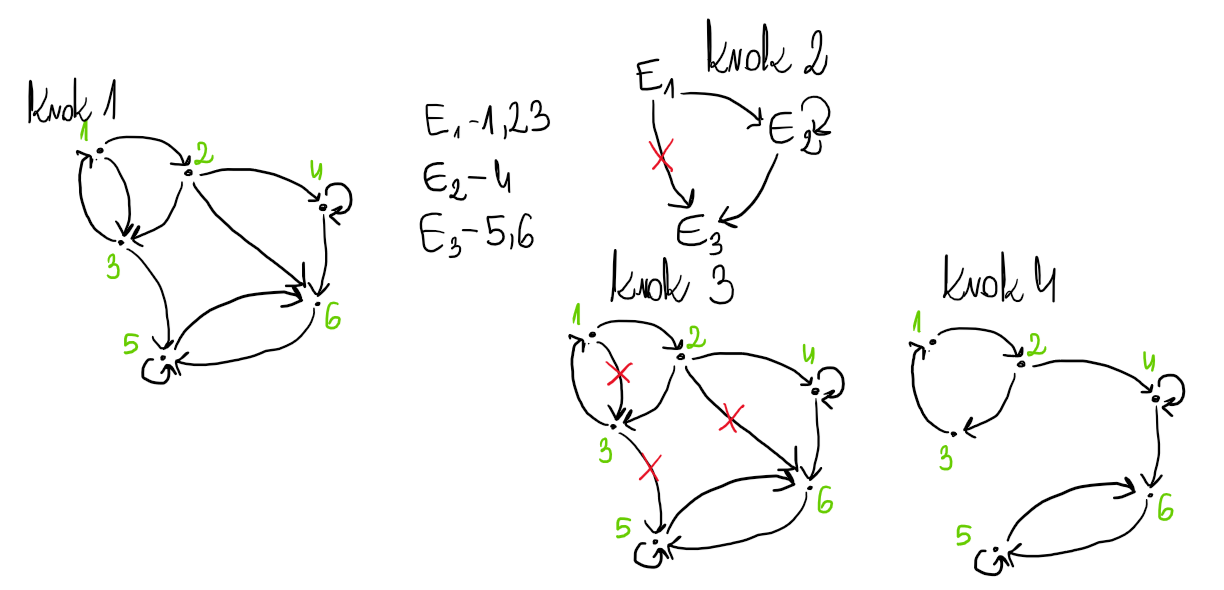
\includegraphics[scale=0.5]{img/redukt2.png}

        Przykład 2
    \end{center}

    \item $ R^*$ -- dopełnienie tranzytywno-zwrotne tj. $ R^* = (R^+)^= $
    \item $ R^{\equiv} $ -- dopełnienie równoważnościowe -- sprawiamy, że relacja staje się relacją równoważności,
    czyli robimy najpierw zwrotną a potem przechodnią, przy okazji symetryczną
\end{enumerate}

Ważne : redukt tranzytywny nie musi się zawierać w relacji pierwotnej, ponieważ tak jak na przykładzie ze zdjęcia, strzałka może iść zamiast z 3 do 5 to może iść
z 1 do 5 co przeczy zawieraniu się. \bigskip

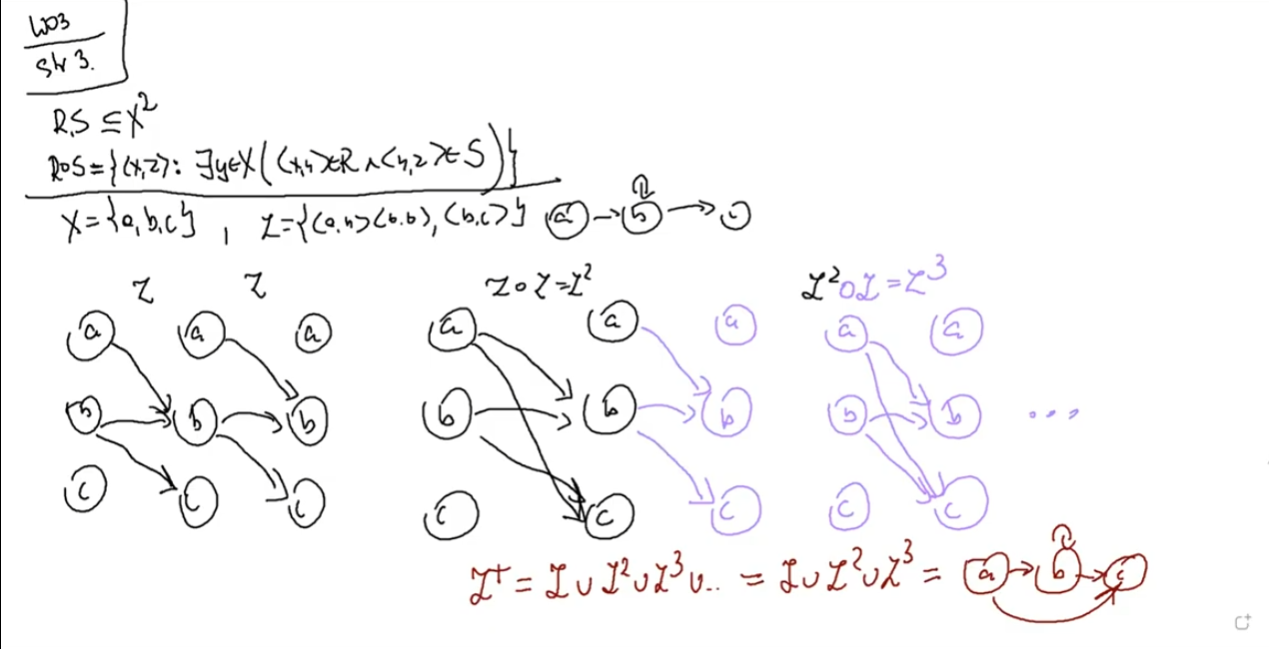
\includegraphics[scale=0.5]{img/zlozenierelacji.png}